\documentclass{standalone}
\usepackage{tikz} % tikz
\usepackage{standalone} % tikz figures are often in standalone
\usepackage{amsfonts} % mathbb etc
\usepackage{amsmath} % crucial package
\usepackage{amsthm} % ams-style theorems
\usepackage{bm} % bold math symbols
\usepackage{xcolor} % more colors
\usepackage[T1]{fontenc} % modern encoding, better than OT1, the default

\newtheorem{definition-fr}{Définition}
\newtheorem{example-fr}{Exemple}
\newtheorem{theorem-fr}{Théorème}
\newtheorem{proposition-fr}{Proposition}
\newtheorem{lemma-fr}{Lemme}
\newtheorem{remark-fr}{Remarque}
\newtheorem{definition}{Definition}
\newtheorem{lemma}{Lemma}
\newtheorem{proposition}{Proposition}
\newtheorem{remark}{Remark}

\usetikzlibrary{decorations.pathmorphing} % for snake, zigzag...
\usetikzlibrary{positioning} % for the "below of=1cm" type of options
\usetikzlibrary{intersections} % e.g. for pyramid
\usetikzlibrary{calc} % for computing node coordinates from others
\usetikzlibrary{overlay-beamer-styles} % when \pause glitches in tikz beamer
\usetikzlibrary{arrows} % arrows
\usetikzlibrary{external} % only compile the figure the first time
\tikzexternalize[only named=true, prefix=tikz-cache/]
\immediate\write18{mkdir -p latex-build/tikz-cache}

% used to pass "scale=XX" as includetikz option
\pgfkeys{
  /tikzoptions/.is family, % Namespace
  /tikzoptions/.cd, % Namespace
  scale/.store in=\scale, % Store the value of 'scale'
}

% usage: \includetikz[scale=XX]{fig}, fetches from my local database
\newcommand{\includetikz}[2][scale=1]{
  \bgroup
  \pgfkeys{/tikzoptions,#1} % currently only accepts 'scale' (april 9 2025)
  \tikzsetnextfilename{#2}
  \include{tex-macros/tikz-figures/#2}% Include the standalone TikZ file
  \egroup
}

% usage: \inputtikz[scale=XX]{fig}, fetches from my local database
\newcommand{\inputtikz}[2][scale=1]{
  \bgroup
  \pgfkeys{/tikzoptions,#1} % currently only accepts 'scale' (april 9 2025)
  \tikzsetnextfilename{#2}
  \input{tex-macros/tikz-figures/#2}% Include the standalone TikZ file
  \egroup
}


\newcommand{\bigOt}{\widetilde{\mathcal{O}}}
\newcommand{\bigO}{\mathcal{O}}

\definecolor{mypurp}{HTML}{8f0c97}
\definecolor{myred}{HTML}{9f103b}
\definecolor{myor}{HTML}{ae3011}
\definecolor{mydarkor1}{HTML}{96240f}
\definecolor{mydarkor2}{HTML}{7f180c}
\definecolor{mylb1}{HTML}{00557e}
\definecolor{mylb2}{HTML}{013157}
\definecolor{mybl1}{HTML}{0d08a9}
\definecolor{mybl2}{HTML}{04037f}
\definecolor{mygr1}{HTML}{097e3e}
\definecolor{mygr2}{HTML}{025520}
\definecolor{myyellow}{HTML}{FFD700}



\makeatletter
\@ifundefined{scale}{
  \def\scale{1}
}
\makeatother


\begin{document}
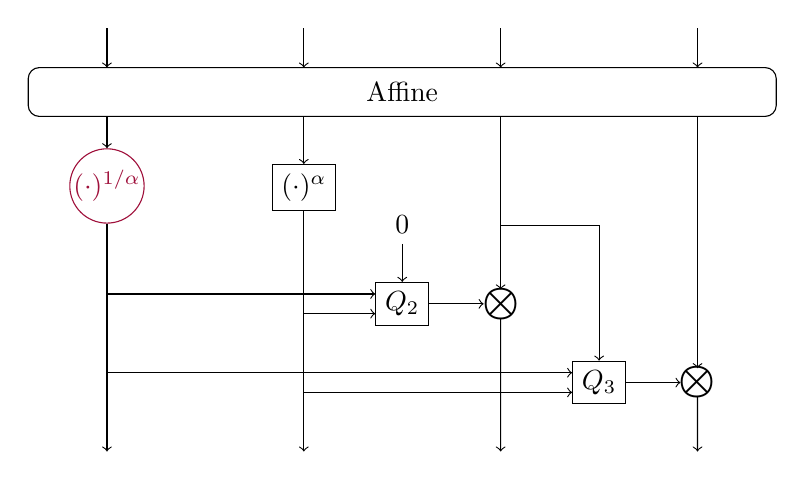
\begin{tikzpicture}[scale=\scale]
  \foreach \z in {0,...,3} {
    \node[] (x\z) at ($\z*(2.5cm,0)$)  {};
    \node[] (y\z) at ($(\z*2.5cm,-4.5)$) {};
  }

  \draw[rounded corners] (-1cm,-.12cm) rectangle node {Affine} (8.5cm,.5cm);

  
  \node[circle,draw,myred,inner sep=0pt] (Pow1) [below=.4cm of x0, draw, distance=3cm] {$(\cdot)^{1/\alpha}$};
  \node (Pow2) [below=.6cm of x1, draw, distance=3cm] {$(\cdot)^\alpha$};
  
  \node[draw] (Q1) at ($(3.75cm,-2.5cm)$) {$Q_2$};
  \node[draw] (Q2) at ($(6.25cm,-3.5cm)$) {$Q_3$};
  
  \node (M1) at (Q1 -| y2) [scale=1.5, inner sep = -0.02cm] {$\bm{\otimes}$};
  \node (M2) at (Q2 -| y3) [scale=1.5, inner sep = -0.02cm] {$\bm{\otimes}$};
  \node (O) [above of = Q1, node distance = 1cm] {$0$};
  
  \node (B1) at ($(0cm, -2.375cm)$) {};
  \node (B2) at ($(2.5cm, -2.625cm)$) {};
  
  \node (B3) at ($(0, -3.375cm)$) {};
  \node (B4) at ($(2.5cm, -3.625cm)$) {};
  
  \node[above of = M1, distance = 2cm] (B5) {};
  
  \draw[->] (x0) -- (Pow1);
  \draw[->] (x1) -- (Pow2);
  \draw[->] (x2) -- (M1);
  \draw[->] (x3) -- (M2);

  \foreach \z in {0,...,3} {
    \draw[->] (\z*2.5cm,1cm) -- (\z*2.5cm,.5cm);
  }
  
  \draw[->] (Pow1) -- (y0);
  \draw[->] (Pow2) -- (y1);
  \draw[->] (M1) -- (y2);
  \draw[->] (M2) -- (y3);
  
  \draw[->] (B1.center) -- (B1.center -| Q1.west);
  \draw[->] (B2.center) -- (B2.center -| Q1.west);
  \draw[->] (B3.center) -- (B3.center -| Q2.west);
  \draw[->] (B4.center) -- (B4.center -| Q2.west);
  \draw[->] (O) 	-- (Q1);
  \draw[->] (B5.center) -- (B5.center -| Q2) -- (Q2);
  \draw[->] (Q1) -- (M1);
  \draw[->] (Q2) -- (M2);
\end{tikzpicture}
\end{document}
